\section{Kernel Regression and Linear Smoothers} 

  K nearest neighbor regression puts equal weights on both near and far points, as long as they are in the window. This may not be ideal, so a simple modification is to \textit{weigh} these points according to their distance from the middle $x$. We can do this with a kernel, as the name suggests. Now this is not the same thing as a Mercer kernel in RKHS, so to distinguish that I will call it a \textit{local averaging kernel}. 

  \begin{definition}[Local Averaging Kernel]
    A \textbf{kernel} is any smooth, symmetric, and non-negative function $K : \mathbb{R} \to \mathbb{R}$.  
  \end{definition}

  \begin{definition}[Kernel Regression]
    Given some datapoints, $X$, our fitted regressor is of form 
    \begin{equation}
      \hat{f} (X) = \frac{\sum_{i} Y_i K \bigg( \frac{||X - X_i||}{h} \bigg)}{\sum_{i} K \bigg( \frac{||X - X_i||}{h} \bigg)}
    \end{equation}
    where $h$ is the \textbf{bandwidth} and the denominator is made sure so that the coefficients sum to $1$. To get a clearer picture, we are really taking the weighted average of the $Y_i$'s. 
    \begin{equation}
      \hat{f} (X) = \sum_{i} Y_i \ell_i (X) \text{ where } \sum_{i} \ell_i (X) = 1
    \end{equation}
    Denoting $Y = (Y_1, \ldots, Y_n) \in \mathbb{R}^n$ and the vector $f(X) = (f(X_1), \ldots, f(X_n))$, if we can write the kernel function as $\hat{Y} = \hat{f}(X) = S Y$, which in matrix form, is 
    \begin{equation}
      \begin{bmatrix} \hat{Y}_1 \\ \vdots \\ \hat{Y}_n \end{bmatrix} = \begin{bmatrix} \hat{f}(X_1) \\ \vdots \\ \hat{f} (X_n) \end{bmatrix} = \begin{bmatrix} \ell_1 (X_1) & \cdots & \ell_n (X_1) \\ \vdots & \ddots & \vdots \\ \ell_1 (X_n) & \cdots & \ell_n (X_n) \end{bmatrix} \begin{bmatrix} Y_1 \\ \vdots \\ Y_n \end{bmatrix} 
    \end{equation}
    then we say that we have a \textbf{linear smoother}, with stochastic matrix $S$ being our \textbf{smoothing matrix}. 
  \end{definition}

  The reason we'd like to have the weights to sum to $1$ is that if we had data that was constant (i.e. all $Y_i$'s are the same), then the fitted function should be constant at that value as well. Furthermore, the theme of linearity is important and will be recurring. The kernel estimator is defined for all $X$, but it's important to see its behavior at the training points $X_i$. The estimator $\hat{Y} = \hat{f}(X)$ is a linear combination of the $Y_i$'s, and the coefficients $\ell_i (X_j)$ depend on the values of $X_j$. Therefore, we have $\hat{Y} = S Y$, which is very similar to the equation $\hat{Y} = H Y$ in linear regression, where $H$ is the hat matrix that projects $Y$ onto the column space of $X$. Nonparametric regression has the same form, but rather than being a projection, it is a linear smoothing matrix. Therefore, this theme unifies both linear regression and nonparametric regression. Linear smoothers, spline smoother, Gaussian processes, are all just different choices of the smoothing matrix $S$. However, not all nonparametric estimators are linear smoothers, as we will see later. 

  Here are some popular kernels. 

  \begin{definition}[Gaussian Kernel]
    The \textbf{Gaussian kernel} is defined as 
    \begin{equation}
      K(x) = \frac{1}{\sqrt{2 \pi}} e^{-x^2/2}
    \end{equation}
    \begin{figure}[H]
      \centering 
      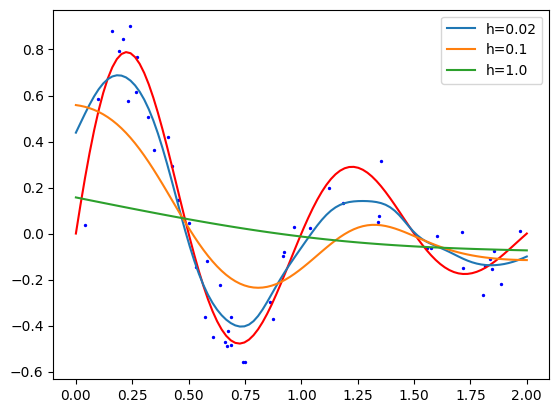
\includegraphics[scale=0.6]{img/gaussian_smoother.png}
      \caption{Gaussian kernel. } 
      \label{fig:gaussian_smoother}
    \end{figure}
  \end{definition}

  \begin{definition}[Box-Car Kernel]
    The \textbf{Box-Car kernel} is defined as 
    \begin{equation}
      K(x) = \frac{1}{2} \mathbbm{1}(|x| \leq 1)
    \end{equation}
    \begin{figure}[H]
      \centering 
      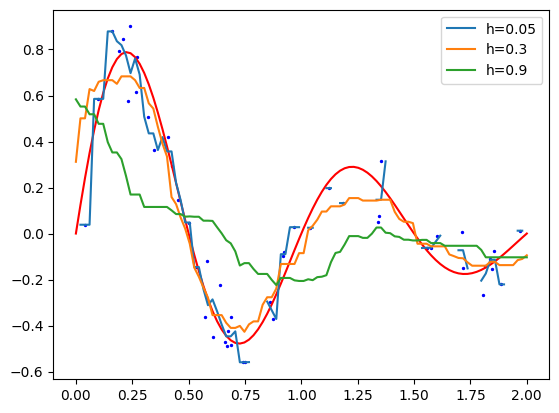
\includegraphics[scale=0.6]{img/boxcar_smoother.png}
      \caption{Boxcar kernel. } 
      \label{fig:boxcar_smoother}
    \end{figure}
  \end{definition}

  \begin{definition}[Epanechnikov Kernel]
    The \textbf{Epanechnikov kernel} is defined as 
    \begin{equation}
      K(x) = \frac{3}{4} (1 - x^2) \mathbbm{1}(|x| \leq 1)
    \end{equation}
    \begin{figure}[H]
      \centering 
      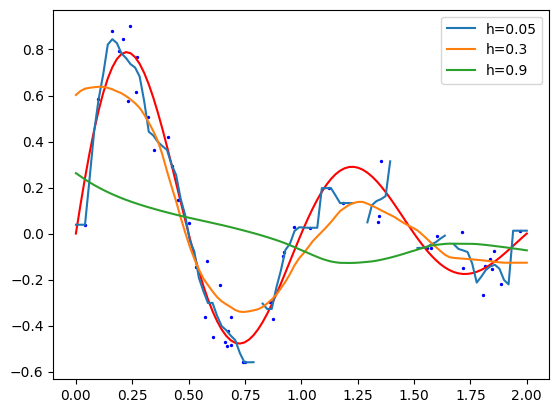
\includegraphics[scale=0.6]{img/epanechnikov_smoother.png}
      \caption{Epanechnikov kernel.} 
      \label{fig:epanechnikov_smoother}
    \end{figure}
  \end{definition}

  It turns out that from a theoretical point of view, the choice of the kernel doesn't really matter. What really matters is the bandwidth $h$ since that is what determines the bias variance tradeoff. To see why, if $h = 0$, then it will simply interpolate the points and variance is extremely high, and if $h = \infty$, then the fitted function will be constant at $\bar{Y}$, leading to high bias. The following theorem formalizes this.  

  \begin{theorem}[Bias Variance Tradeoff of Kernel Regression]
    Suppose that $d = 1$ and that $m^{\prime\prime}$ is bounded. Also suppose that $X$ has a nonzero, differentiable density $p$ and that the support is unbounded. Then, the risk is 
    \begin{align}
      R_n & = \frac{h_n^4}{4} \bigg( \int x^2 K(x) \bigg)^2 \int \bigg( m^{\prime\prime} (x) + 2m^\prime (x) \frac{p^\prime (x)}{p(x)} \bigg)^2 \,dx \\
          & \;\;\; + \frac{\sigma^2 \int K^2(x)\,dx} {n h_n} \int \frac{dx}{p(x)} + o \bigg( \frac{1}{n h_n} \bigg) + o(h_n^4) 
    \end{align}
    The first term is the squared bias and the second term is the variance. 
  \end{theorem}
  \begin{proof}
    We first denote 
    \begin{equation}
      \hat{f}(X) = \frac{\frac{1}{nh} \sum_{i=1}^n K \bigg( \frac{X - X_i}{h} \bigg) Y_i}{\frac{1}{nh} \sum_{i=1}^n K \bigg( \frac{X - X_i}{h} \bigg)} 
    \end{equation}
    where the denominator is the kernel density estimator $\hat{p}(X)$. Therefore, we rewrite
    \begin{align}
      \hat{f} (x) - f(x) & = \frac{\hat{a}(x)}{\hat{p}(x)} - f(x) \\
                         & = \bigg( \frac{\hat{a}(x)}{\hat{p}(x)} - f(x) \bigg) \bigg( \frac{\hat{p}(x)}{p(x) + 1 - \frac{\hat{p}(x)}{p(x)}} \bigg) \\
                         & = \frac{\hat{a}(x) - f(x) \hat{p}(x)}{p(x)} + \frac{(\hat{f}(x) - f(x)) (p(x) - \hat{p}(x))}{p(x)}
    \end{align}
    as $n \rightarrow \infty$ both $\hat{f}(x) - f(x)$ and $p(x) - \hat{p}(x)$ going to $0$, and since they're multiplied in the second term, it will go to $0$ very fast. So the dominant term is the first term, and we can write the above as approximately 
    \begin{equation}
      \hat{f}(x) - f(x) \approx  \frac{\hat{a}(x) - f(x) \hat{p}(x)}{p(x)}
    \end{equation}
    TBD continued. Wasserman lecture 6, 10:00. 
  \end{proof}

  From the theorem above, we can see that if the bandwidth is small, then $h^4$ is small and the bias decreases. However, there is a $h$ term in the denominator of the variance term, which also trades it off. We can furthermore see that the bias is sensitive to $p^\prime / p(x)$. This means that if the density is steep, then the bias will be high. This is known as \textit{design bias}, which is an underlying weakness in smoothing kernel regression. Another problem that is not contained in the theorem is the \textit{boundary bias}, which states that if you're near the boundary of the distribution (i.e. near the boundary of its support), then the bias also explodes. This happens to be very nasty especially in high dimensions where most of the data tends to be near the boundary. It turns out that this can be easily fixed with local polynomial regression, which gets rid of this term in the bias without any cost to variance. This means that this is unnecessary bias. 

  Then you can apply regularization on this to get kernel ridge regression. 

  \begin{code}[MWS of Kernel Ridge Regression in scikit learn]
    \begin{lstlisting}
      from sklearn.kernel_ridge import KernelRidge
      import numpy as np
      n_samples, n_features = 10, 5
      rng = np.random.RandomState(0)
      y = rng.randn(n_samples)
      X = rng.randn(n_samples, n_features)
      krr = KernelRidge(alpha=1.0)
      krr.fit(X, y)
    \end{lstlisting}
  \end{code}

